

We describe our methodology and experiment setup in Section~\ref{ssec:methodology}, and present our results 
in Section~\ref{ssec:results}.

\subsection{Methodology}
\label{ssec:methodology}

\paragraph{Evaluated systems.}

We compare \sys\  to  state-of-the art TPSs and separately evaluate the effectiveness of its FP mechanism.
To this end, we compare four TPSs, all of which use HBase as the underlying data store -- Omid, \sysll, 
\syspc, and \sys. \syspc\ defers writes to commit time (as Percolator does), whence it writes and validates
keys using check\&mutate.
\remove{
\begin{description}
\item[\sys] -- the algorithm described in Section~\ref{sec:ll}, without support for FP transactions.
\item[\sys] -- single-key transactions use the FP API, 
whereas longer transactions use the standard API, 
and their transactional reads and writes are modified to access the LVC along with the data as described in Section~\ref{sec:alg}.
\item[Omid] -- the Apache Incubator version of Omid, on which we base our implementation of \sys. 
\item[2PC] -- an implementation (in the \sys\ framework) of Percolator's concurrency control mechanism:
Begins and commits use the TM only for timestamp allocation and not for conflict detection; conflicts are detected via 
\emph{Two Phase Commit (2PC)}.
\end{description}
}
In \sys, single-key transactions use the FP API, whereas longer transactions use the standard API. 
The other systems use the standard API only.

Note that both CockroachDB and Percolator use 2PC-based conflict resolution, so our \syspc\ mimics
their protocols. 
Direct comparison with the actual systems is not feasible because Percolator is proprietary and 
CockroachDB supports SQL transactions over a multi-tier
architecture using various components that are incompatible with HBase. 
We also do no compare \sys\ to Omid1 (and the similarly-designed Tephra), since Omid significantly
outperforms Omid1~\cite{Omid2017}.

To reduce latency, we configure the TPSs to perform the post-commit phase asynchronously, 
by a separate thread, after the transaction completes.

\remove{
In Omid and Vanilla \sys, all transactions use the standard API, namely 
delineating transactions with begin and commit calls.
In FP \sys, transactions that can use the FP API (specifically, singleton reads, singleton writes, 
and single-key read-writes) do so, whereas other transactions use the standard API.
}

\paragraph{Experiment setup.}

Our experiment testbed consists of nine 12-core Intel Xeon 5 machines with 46GB RAM and 4TB 
SSD storage, interconnected by 10G Ethernet. We allocate three of these to HBase nodes, 
one to the TM, one to emulate the client whose performance we measure, and four more to simulate 
background traffic as explained below. Each HBase node runs both an HBase region server and 
the underlying Hadoop File System (HDFS) server within 8GB JVM containers. 

Note that the only scalability bottleneck in the tested systems is the centralized TM.
HBase, on the other hand, can scale horizontally across thousands of nodes, each of which processes a small fraction of the total load. 
Since each node typically serves millions of  keys, data access rates remain load-balanced across nodes 
even when access to individual keys is highly skewed.  And since read/write requests are processed independently by each HBase node, 
their performance remains constant as the workload and  system size are scaled by the same factor. 

Thus, to understand the system's performance at scale, 
we can run transactions over a small HBase cluster with an appropriately-scaled load, 
but need to stress the TM as a bigger deployment would. 
We do this at a ratio of 3:1000; that is, we run transactions on a $3$-node HBase cluster and 
load the TM with a begin/commit request rate that would arise in a $1000$-node HBase cluster with the same per-node load.
For example, to test the client's latency at $100$K tps, we have the TM handle $100$K tps, and have  an HBase deployment of
three nodes handle read/write requests of $300$ tps. As explained above, 
the HBase latency at $100$K tps with $1000$ servers would be roughly the same as in this deployment.

We use four machines to generate the background load on the TM using a custom tool~\cite{Omid2017} 
that asynchronously posts begin and commit requests on the wire and collects the TM's responses. 
We note that although in this experiment the TM maintains a small number of client connections (serving many requests per connection), 
the number in a true $1000$-node system still falls well within the OS limit, hence no real bottleneck is ignored. 

We measure the end-to-end client-incurred latency on a single client node that generates transactions over the $3$-server HBase cluster. 
Note that the client also generates begin/commit requests, which account for \mbox{$\sim0.3\%$} of the TM's load.
The client runs the popular YCSB benchmark~\cite{Cooper:2010:BCS:1807128.1807152}, 
exercising the synchronous transaction processing API in a varying number of threads. 

\paragraph{Workload.}

Our test cluster stores approximately 23M keys ($\sim\!\!7$M keys per node). 
The values are 2K big, yielding roughly 46GB of actual data, replicated three-way in HDFS. The keys are hash-partitioned
across the servers. The data accesses are 50\% reads and 
50\% writes. The key access frequencies follow a Zipf distribution, generated following 
the description in~\cite{Gray:1994:QGB:191839.191886}, with $\theta=0.8$, which we derive from production 
workloads. In this distribution, the first key is accessed 0.7\% of the  time.
%in Yahoo's deployment of Omid~\cite{Omid2017}. 
%Note that under this access distribution, data requests are load-balanced across nodes.

\noindent
We test the system with two transaction mixes:
\begin{description}
\item[Random mix] -- 
transaction sizes (number of reads and writes) follow a Zipf distribution with $\theta=0.99$, with a cutoff at $10$. 
With these parameters, $63\%$ of the transactions access three keys or less, and only $3\%$ access $10$ keys. 
We vary the system load from 30K to 500K transactions per second (tps). 
\item[BRWC] -- $80\%$ of the transactions are drawn from the random mix distribution, and $20\%$ perform a read
and then a write to the same key. 
\end{description}

We add the BRWC workload since single-key read+write transactions are common in production, but are highly unlikely to 
occur in our random mix, which uses random key selection with billions of keys.

\begin{figure}[htb]
	\centering
      	\includegraphics[width=0.48\textwidth]{figs/throughputlatency1.pdf}
	    \caption{Throughput vs.\ latency, transaction size = 1.}
        \label{fig:tl-1}      
\end{figure}


\begin{figure*}[hbt]
\centering
\begin{tabular}{ccc}
      \begin{subfigure}[t]{0.48\textwidth}
         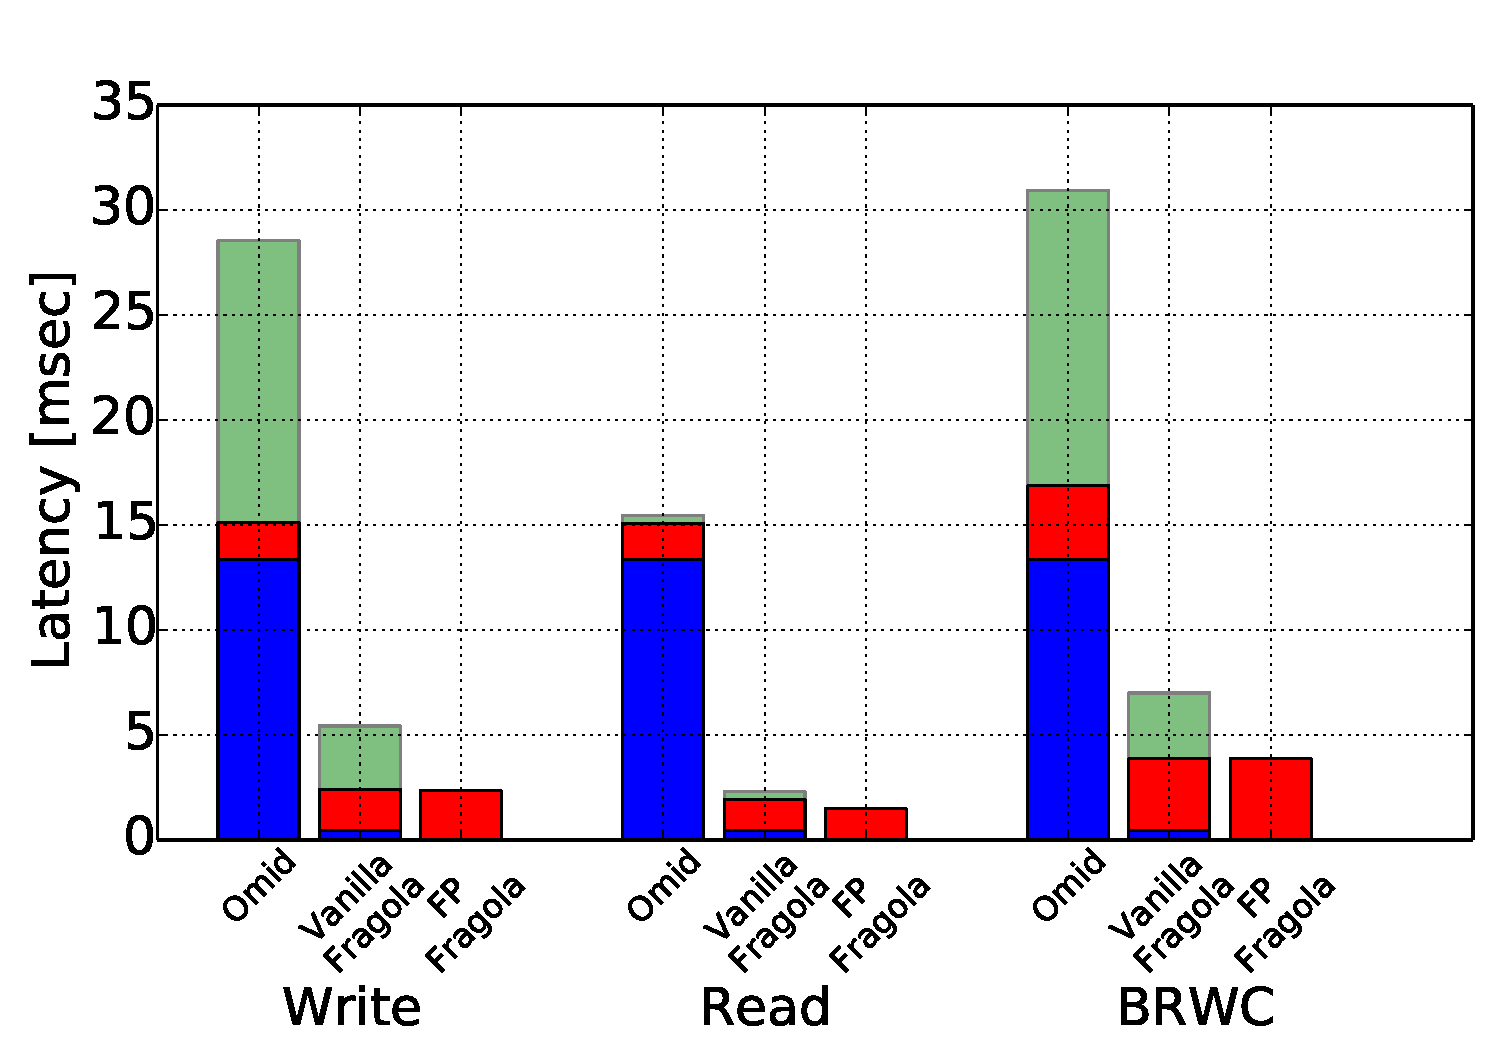
\includegraphics[width=\textwidth]{figs/latency_allPUTGET.pdf}
        \caption[]{Low load (100K tps).}
        \label{fig:stack-brc}

      \end{subfigure} 
    
& 
      \begin{subfigure}[t]{0.48\textwidth}
      	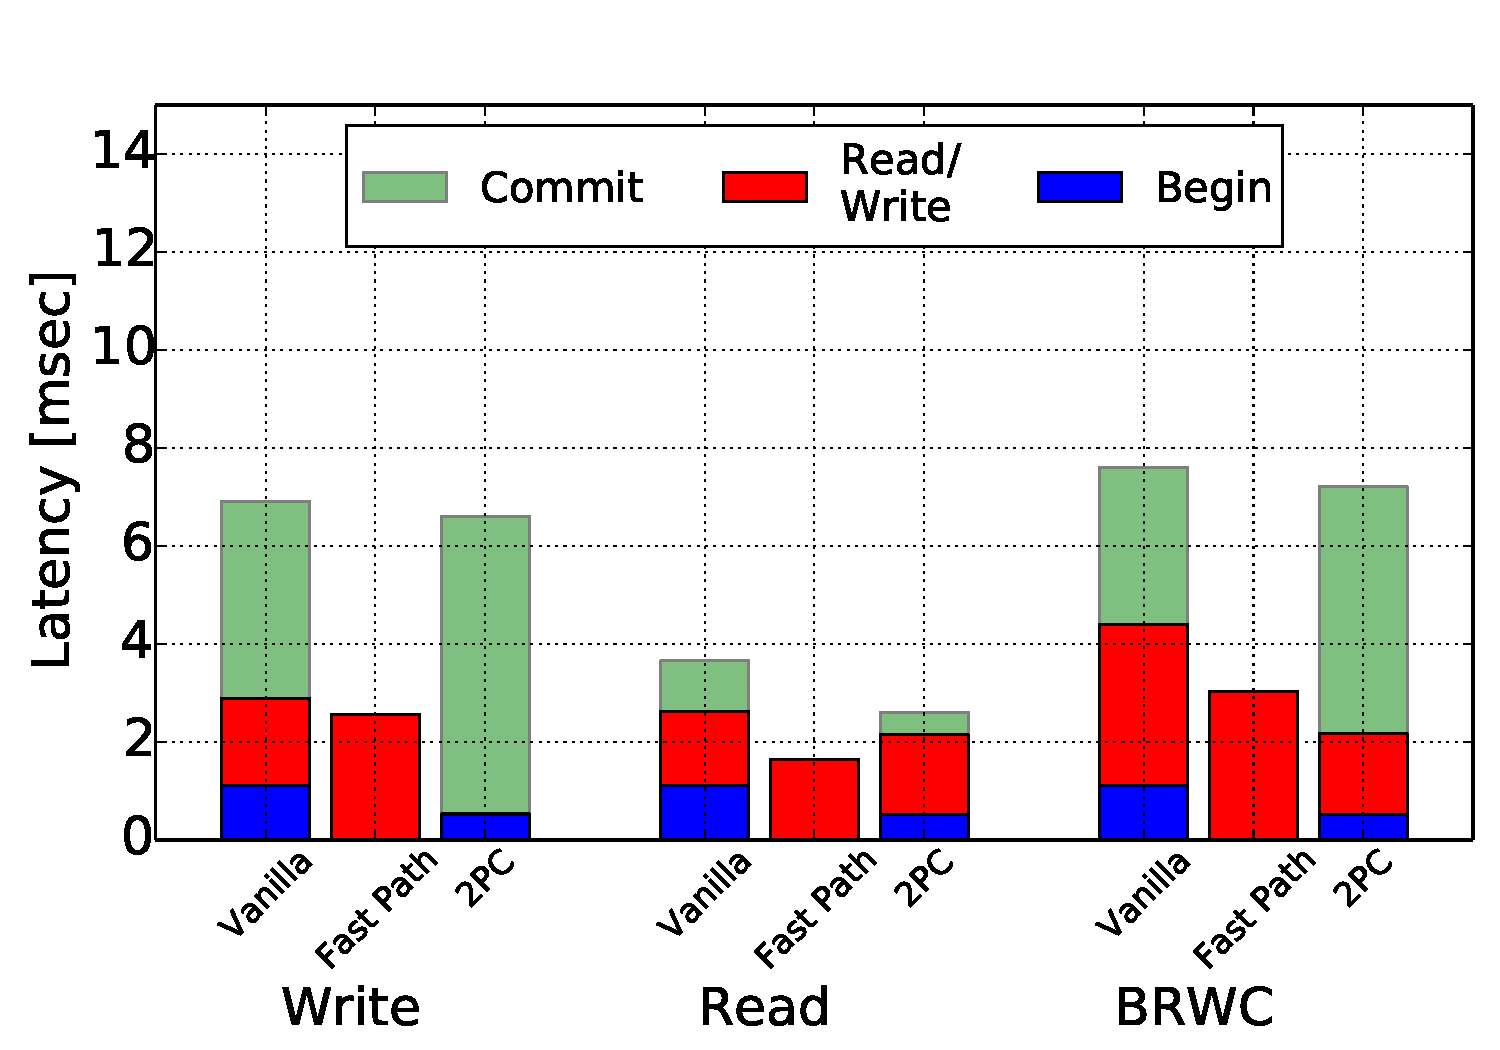
\includegraphics[width=\textwidth]{figs/latencyHighThrough_PUTGETRMW.pdf}
	\caption{High load (500K tps).}
	\label{fig:hightx}
      \end{subfigure}  & 

\end{tabular}
       \caption{Latency breakdown  for single-key transactions under  random mix workload. }
\end{figure*}


\subsection{Results}
\label{ssec:results}

\mypara{Throughput and latency of short transactions.} 
%
Recall that \sys\ is motivated by the prevalence of short transactions in production, and is designed with
the goal of accelerating such transactions.
Its advantage is less pronounced for long transactions, where the cost of begin and commit is amortized
across many reads and writes.
To make the comparison meaningful, we classify transactions by their lengths and whether they
access a single key, and study each transaction class separately. 

We begin with short transactions. 
Figure~\ref{fig:tl-1} presents the average latency of single-key transactions run as part of the random mix,
as a function of {system} throughput.
Figure~\ref{fig:stack-brc}  then zooms in on the latency of such transactions under 
a throughput of 100K tps, and breaks up the different factors contributing to it. 
Figure~\ref{fig:hightx}  presents a similar breakdown under a high load of 500K tps; Omid 
is not included since it does not sustain such high throughput.

As we can see, under light load, \sysll\ and \syspc\ improve the latency of Omid by 4x to 5x.
%, even without the fast path.
This is because in Omid, both begin and commit wait for preceding transactions to complete the writes of 
their commit entries; this stems from Omid's design choice to avoid the need for resolving pending write intents
by aborting transactions; see penultimate column in Table~\ref{table:design-space}. 
Single-key writes suffer from both the begin and commit latencies, whereas single-key reads  
suffer only from begins (Figure~\ref{fig:stack-brc}). \syspc\ has longer commit latencies and shorter write latencies
because it defers writes to commit time.

As load increases, Omid suffers from a well-pronounced bottleneck, and its latency at 250K tps is doubled, where the other systems
are unaffected. The extra delay in Omid is due to batching of commit record updates, 
which its TM applies to handle congestion~\cite{Omid2017}. 

Under low load, \sysll\ is slightly faster than \syspc\ (due to the latter's use of atomic check\&mutate). 
But under high load, \syspc\ is slightly better ($10\%$ faster on average for single-key transactions)   
due to the centralized conflict analysis becoming a bottleneck in \sysll.

The FP API delivers better performance for this traffic. For instance, under low load (Figure~\ref{fig:stack-brc}),
single writes take an average of 2.4ms using 
the {\code bwc} API versus 5.7ms in \sysll\ (and 5.9ms in \syspc). 
For comparison, a native HBase write takes roughly 2ms under this load.
A single read executed using {\code brc} takes 1.5ms, which is the average latency of a native HBase read,
versus 2.5ms as a regular transaction in \sysll\ (2.7ms in \syspc). 
For transactions that read and write a single key as part of the BRWC workload, 
%Their latency breakdown under a 100K tps throughput is shown in Figure~\ref{fig:rmw}.
the fast path implementation (consisting of \code{br} and \code{wc} calls) completes within 4ms,
versus 6.5ms for  \sysll, 7.1ms for \syspc, and 37.6ms for Omid. 
%
Under high load (Figure~\ref{fig:hightx}), the fast path is even more beneficial: it reduces the latency of 
both read and write by more than a factor of 2. 
%2.7, from 6.9ms  to 2.6ms, and the read latency by a factor of 2.2, from  3.7ms to 1.7ms.
%, read, and brwc from 11.24ms, 8.24ms, and 11.85ms to 2.4ms, 1.29ms, and 4.19ms respectively. 



\mypara{Long transactions.} 
We now examine longer transactions run as part of the random mix.
Figure~\ref{fig:throughput-latency} shows the results for transactions of lengths $5$ and $10$.
We see that the absolute latency gap of the new systems over Omid remains similar, but is amortized 
by other operations. Omid's control requests (begin and commit) continue to 
dominate the delay, and comprise $68\%$ of the latency of 10-access transactions (under low load).
In contrast, the transaction latency of \sysll\ (and \sys) is dominated by data access, 
as only $13\%$ (resp.~$18\%$)  of the time is spent on the control path. 
\syspc\ spends $66\%$ time executing commit  because it defers writes to commit time,
but this is offset by a shorter read/write execution time.

\begin{figure*}[t]
\centering{
\begin{tabular}{cc}

    \begin{subfigure}[t]{0.48\textwidth}
	\includegraphics[width=\textwidth]{figs/throughputlatency10.pdf}
	\caption[]{Throughput versus latency, transaction size = 10}
    \label{fig:tl-10}
  \end{subfigure} & 


  \begin{subfigure}[t]{0.48\textwidth}
	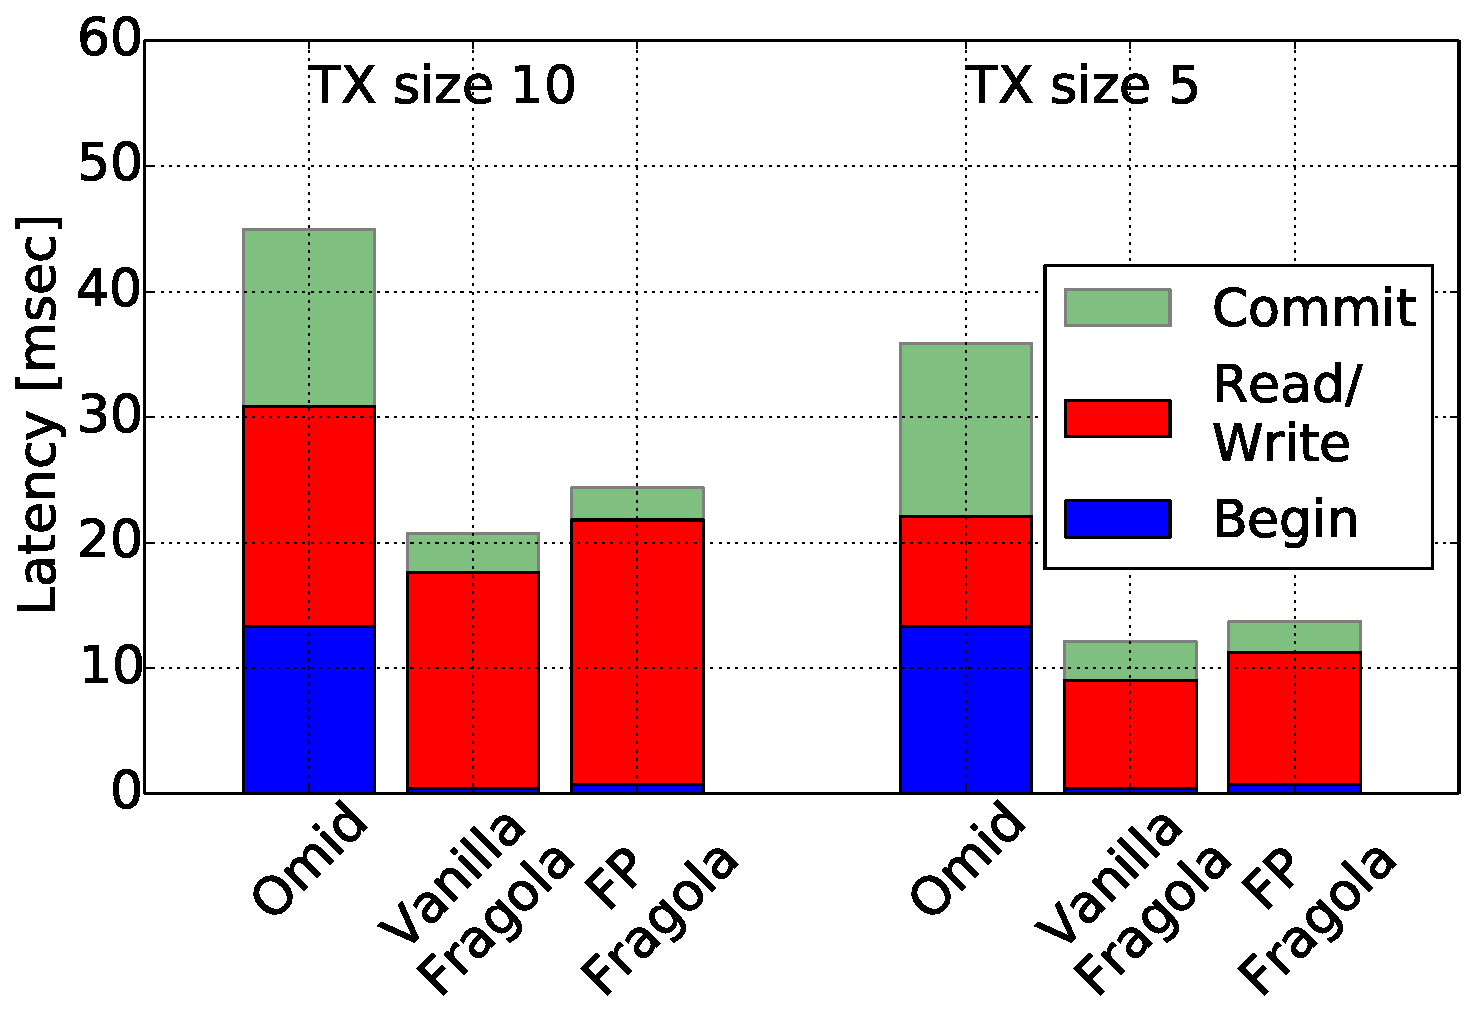
\includegraphics[width=\textwidth]{figs/latency_5_10.pdf}
	\caption[]{Latency breakdown, transaction size = 5, 10}
    \label{fig:stack-tx10}
  \end{subfigure} 
\end{tabular}  	
}		
  \caption{Latency vs.\ throughput  and latency breakdown  for long transactions in random mix workload. }
  \label{fig:throughput-latency}
\end{figure*}



The FP mechanism takes a toll on the data path, which uses atomic check\&mutate operations 
instead of simple writes. This is exacerbated for long transactions.
For example, a 10-access transaction takes 24.8ms with \sys, 
versus 21.7ms with  \sysll. The performance of \syspc\ with long transactions is similar to that of \sys\ -- e.g., 25.6ms for 10-access transactions -- 
because it also uses check\&mutate operations during the commit validation phase.

 

\begin{figure}[h!]
\centering
\begin{subfigure}[t]{0.48\textwidth}
\centerline{
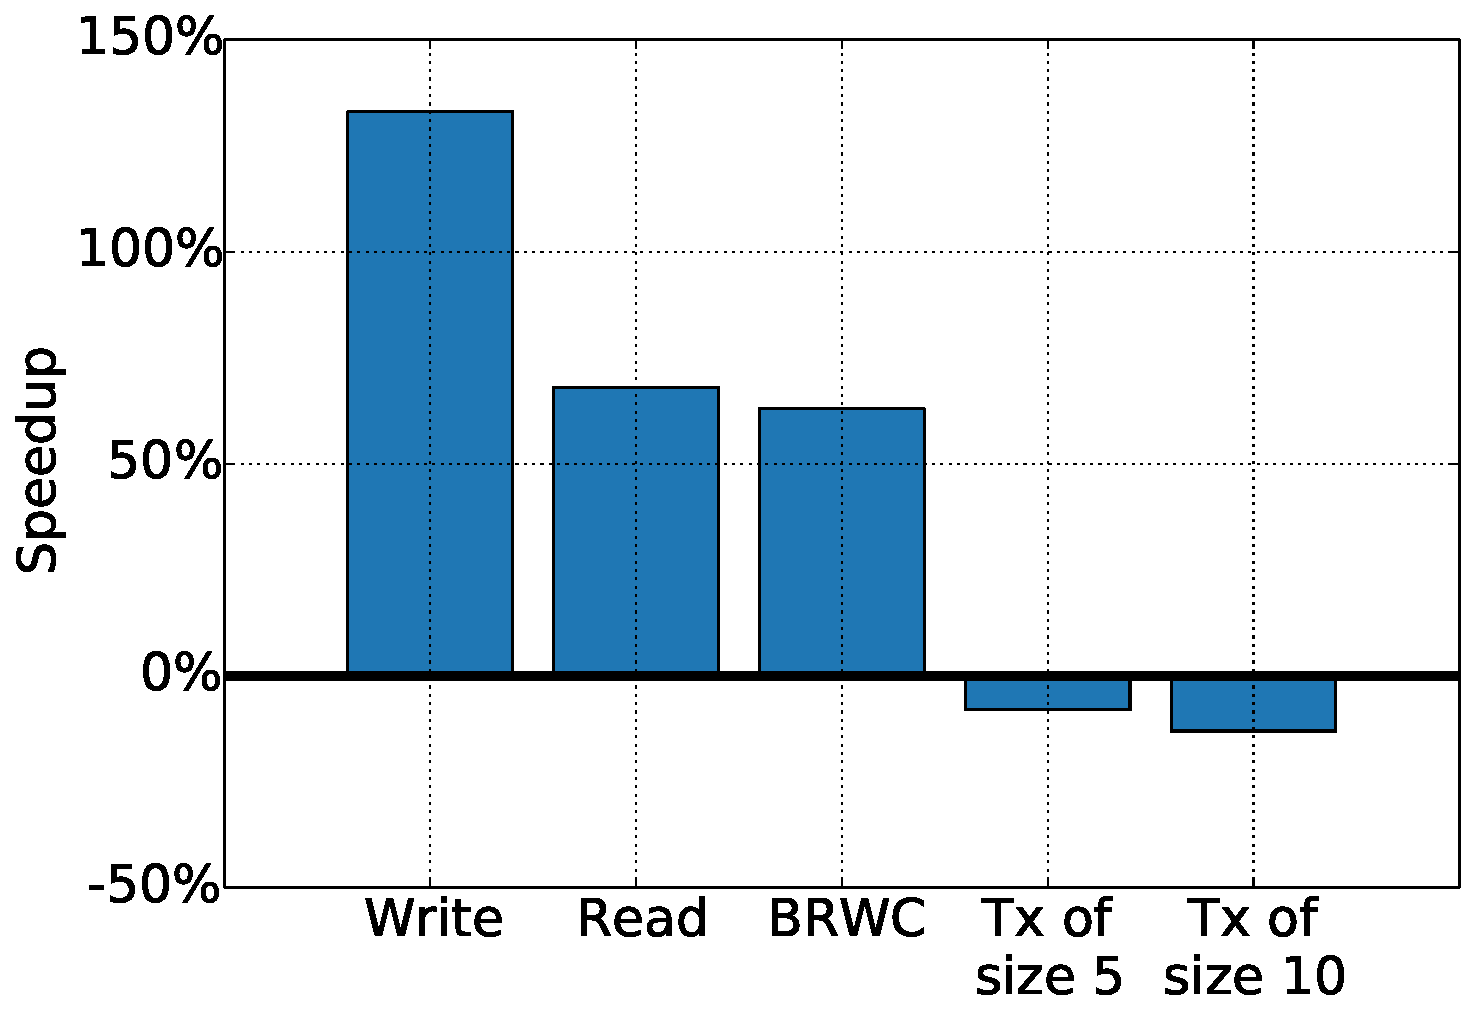
\includegraphics[width=.9\textwidth]{figs/low_speedup.pdf}
}
\caption{Low load (100 tps)} 
\label{fig:slowdown-low}
\end{subfigure} 
\begin{subfigure}[t]{0.48\textwidth}
\centerline{
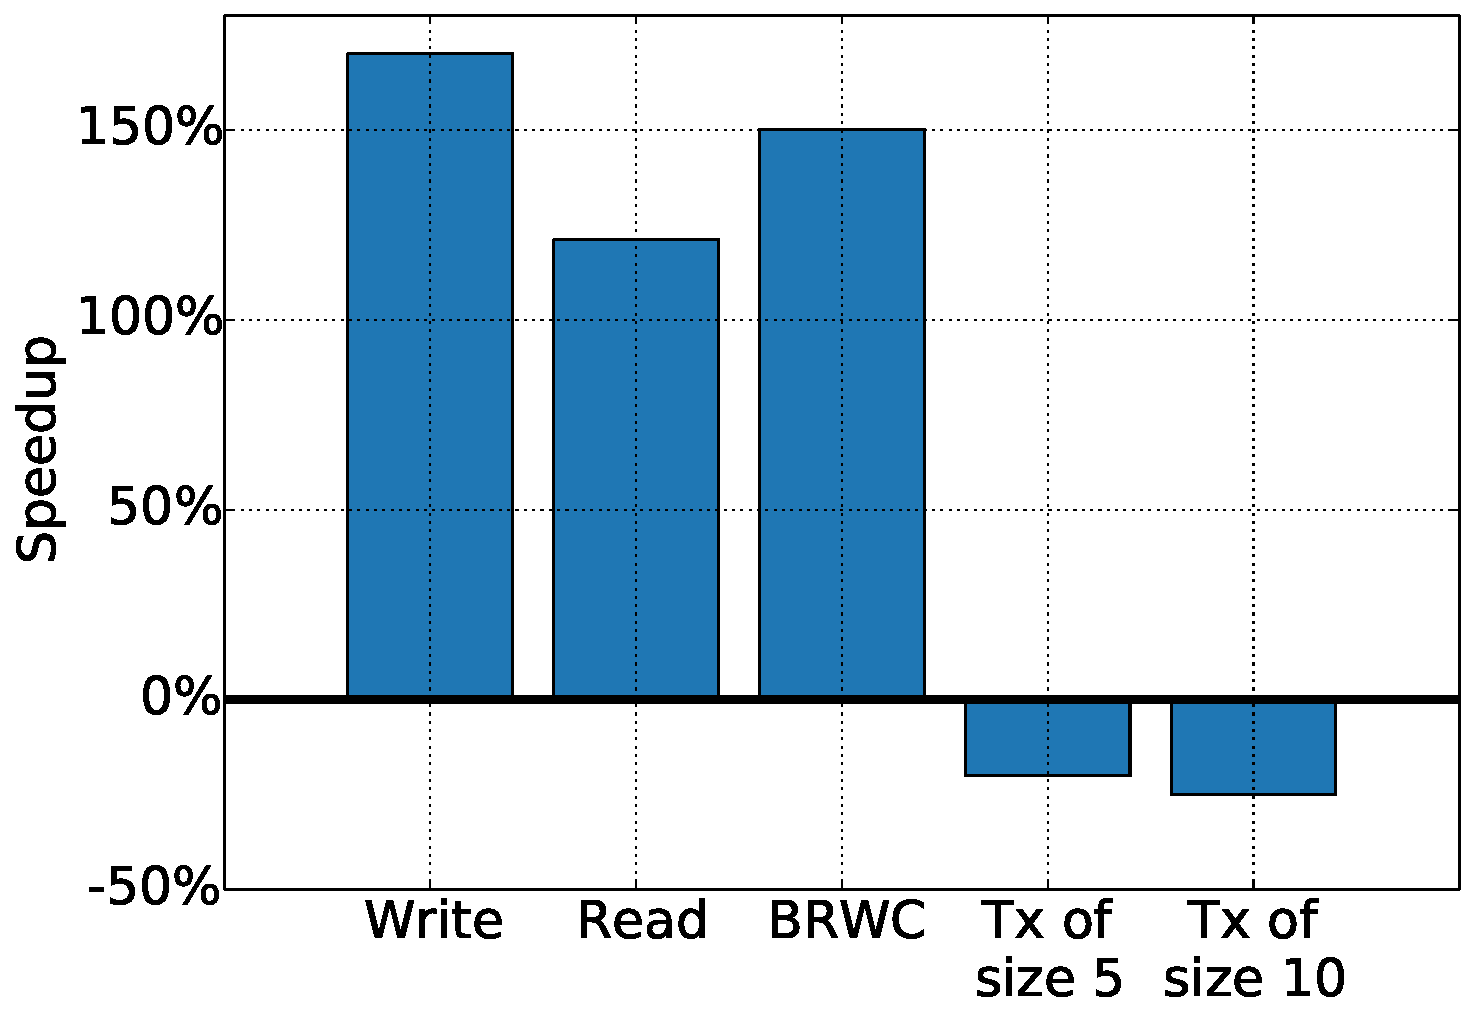
\includegraphics[width=.9\textwidth]{figs/high_speedup.pdf}
}
\caption{High load (500 tps)} 
\label{fig:slowdown-high}
\end{subfigure} 
\caption{Latency speedup with  fast path API in {\sys}.}
\label{fig:fp-tradeoff}
\end{figure}



Figure~\ref{fig:fp-tradeoff} summarizes the tradeoffs entailed by \sys\ relative to \sysll\ for the different transaction classes. 
We see that under low load (Figure~\ref{fig:slowdown-low}),
the speedup for single-write transactions is $2.3$x, whereas the worst slowdown is $13\%$. 
In systems geared towards real-time processing, this is a reasonable tradeoff, since long transactions 
are infrequent and less sensitive to extra delay.
Under high load (Figure~\ref{fig:slowdown-high}), the fast path is even more advantageous: the speedup for writes is $2.7$x.
%In systems geared towards real-time processing, this is a reasonable tradeoff, since long transactions 
%are infrequent and less sensitive to extra delay. Under the studied workload, e.g.,   FP \sys\/ is more desirable. 



\mypara{Abort rates.}

%Abort rates are extremely low -- between  $0.01\%$ and  $0.02\%$ -- for all systems. To Do: try a sharper Zipf.}  
We note that \sys\ yields slightly higher rates of transaction aborts compared to Omid 
(recall that \sysll\ aborts tentative writes in favor of concurrent reads, whereas  \sys\ also aborts
singleton writes in presence of concurrent tentative writes). However, the abort rates exhibited by all  
the systems are minor. 
Here, under the highest contention,  \sys\ aborts approximately $0.1\%$ 
of the transactions versus  \sysll's $0.08\%$,   
 \syspc's $0.08\%$ 
and Omid's $0.07\%$ 
(the latter  is in line with production abort rates reported in Omid~\cite{Omid2017}).  


